\documentclass[12pt, titlepage]{article}

\usepackage{fullpage}
\usepackage[round]{natbib}
\usepackage{multirow}
\usepackage{booktabs}
\usepackage{tabularx}
\usepackage{graphicx}
\usepackage{float}
\usepackage{hyperref}
\hypersetup{
    colorlinks,
    citecolor=black,
    filecolor=black,
    linkcolor=red,
    urlcolor=blue
}
\usepackage[round]{natbib}

\newcounter{acnum}
\newcommand{\actheacnum}{AC\theacnum}
\newcommand{\acref}[1]{AC\ref{#1}}

\newcounter{ucnum}
\newcommand{\uctheucnum}{UC\theucnum}
\newcommand{\uref}[1]{UC\ref{#1}}

\newcounter{mnum}
\newcommand{\mthemnum}{M\themnum}
\newcommand{\mref}[1]{M\ref{#1}}

\title{SE 3XA3: Software Requirements Specification\\KingMe}

\author{Team 9, KingMe
		\\ Ardhendu Barge 400066133
		\\ Dylan Smith 001314410
		\\ Thaneegan Chandrasekara 400022748
}

\date{\today}

\begin{document}

\maketitle

\pagenumbering{roman}
\tableofcontents
\listoftables
\listoffigures

\begin{table}[!ht]
\caption{\bf Revision History}
\begin{tabularx}{\textwidth}{p{3cm}p{2cm}X}
\toprule {\bf Date} & {\bf Version} & {\bf Notes}\\
\midrule
2021/03/10 & 0 & Added the modules of the system\\
2021/03/11 & 0 & Added likely and unlikely changes\\
2021/03/14 & 0 & Added the traceability tables\\
2021/03/18 & 0 & Added the section introducitons\\
\bottomrule
\end{tabularx}
\end{table}

\newpage

\pagenumbering{arabic}

\section{Introduction}

A very important part of the development of our checkers application, King Me, is modular decomposition. This is the process of breaking our application into individual modules each containing one secret. In this document we will be discussing each of these different modules, the secret they contain and how they have been designed for change. We will be discussing the changes we anticipate being made in the future and how the modules have been designed to allow these changes to be easily made, and we will discuss the unlikely changes that we don't anticipate being made. We will be discussing the structure of the modules and how they comprise the system. Lastly we will demonstrate how the requirements are being met by the different modules of our system.

\section{Anticipated and Unlikely Changes} \label{SecChange}
This section will list possible changes that may be made to the system. They will be separated into anticipated and unlikely changes.

\subsection{Anticipated Changes} \label{SecAchange}

Anticipated changes are changes that were anticipated during the design process. These changes influenced the modular decomposition of our system. They are changes that we anticipate will likely be made and should be easily made. We chose to decompose the system into modules containing secrets such that each of these changes would result in the modification of only one module, therefore making it much easier to implement the changes when the time comes. 

\begin{description}
\item[\refstepcounter{acnum} \actheacnum \label{acAlgorithm}:] Modifying the algorithm for generating computer moves.
\item[\refstepcounter{acnum} \actheacnum \label{acGraphics}:] Changing the graphical elements used to display the application.
\item[\refstepcounter{acnum} \actheacnum \label{acMenu}:] The tutorial will need to be updated when new features are added or removed.
\item[\refstepcounter{acnum} \actheacnum \label{acBoard}:] Changes to the implementation of the state of the board.
\item[\refstepcounter{acnum} \actheacnum \label{acMoves}:] Changing how the valid moves are generated.
\item[\refstepcounter{acnum} \actheacnum \label{acRules}:] More advanced checkers rules may be added.
\end{description}

\subsection{Unlikely Changes} \label{SecUchange}

Unlikely changes are those that we do not anticipate being made. The module structure was not be designed to accommodate these changes. They will likely require the modification of multiple modules, making these changes much more difficult to implement.


\begin{description}
\item[\refstepcounter{ucnum} \uctheucnum \label{ucIO}:] The input will come from the mouse and the screen will be used to output to. 
\item[\refstepcounter{ucnum} \uctheucnum \label{ucInput}:] The user is the source of the input.
\end{description}

\section{Module Hierarchy} \label{SecMH}

In this section we discuss our module design. The modules are separated into Hardware-Hiding, Behaviour-Hiding and Software Decision Hiding based on the secrets they contain. 

\begin{description}
\item [\refstepcounter{mnum} \mthemnum \label{mGUI}:] GUI Module
\item [\refstepcounter{mnum} \mthemnum \label{mM}:] Menu Module
\item [\refstepcounter{mnum} \mthemnum \label{mB}:] Board Module
\item [\refstepcounter{mnum} \mthemnum \label{mG}:] GameLogic Module
\item [\refstepcounter{mnum} \mthemnum \label{mP}:] Piece Module
\item [\refstepcounter{mnum} \mthemnum \label{mA}:] AI Module
\end{description}


\begin{table}[h!]
\centering
\begin{tabular}{p{0.3\textwidth} p{0.6\textwidth}}
\toprule
\textbf{Level 1} & \textbf{Level 2}\\
\midrule

{Hardware-Hiding Module} & None \\
\midrule

\multirow{7}{0.3\textwidth}{Behaviour-Hiding Module} & GUI Module\\
& Menu Module\\
& Board Module\\
& GameLogic Module\\
& Piece Module\\
\midrule

\multirow{1}{0.3\textwidth}{Software Decision Module} & AI Module\\
\bottomrule

\end{tabular}
\caption{Module Hierarchy}
\label{TblMH}
\end{table}

\section{Connection Between Requirements and Design} \label{SecConnection}

King Me has been designed to meet the functional and nonfunctional requirements as outlined in the SRS document. Table \ref{TblRT} shows all the requirements of the SRS document alongside the modules used to satisfy them. 

\section{Module Decomposition} \label{SecMD}

In this section we will discuss what modules our system have been decomposed into. We will introduce the different modules and briefly explain their role in the overall system. Each module is broken up into a secret, a service and an implementation. The secret of the module is the design decision that has been hidden within the module , the service of the module is what the module does, and the implementation is how we implemented the module.

\subsection{Hardware Hiding Modules}
%\subsection{Hardware Hiding Modules (\mref{mHH})}
\begin{description}
\item N/A - This implementation contains no hardware hiding modules.
\end{description}

\subsection{Behaviour-Hiding Modules}

\subsubsection{GUI Module (\mref{mGUI})}

\begin{description}
\item[Secrets:] Manages the display of the application.
\item[Services:] Displays the UI to the screen. Displays the board, the pieces and the menu options in the desired configurations. Captures interactions on the UI and relays to appropriate modules.
\item[Implemented By:] GUI.py (Python)
\end{description}

\subsubsection{Menu Module (\mref{mM})}

\begin{description}
\item[Secrets:] Manages the 'New Game' and 'Tutorial' logic.
\item[Services:] Provides a way to restart the game and also provides instructions on how to play the game.
\item[Implemented By:] menu.py (Python)
\end{description}

\subsubsection{Board Module (\mref{mB})}

\begin{description}
\item[Secrets:] Manages the state of the game board.
\item[Services:] Provides details on the state of the game board, including where pieces are located on the board.
\item[Implemented By:] board.py (Python)
\end{description}

\subsubsection{GameLogic Module (\mref{mG})}

\begin{description}
\item[Secrets:] The checkers logic.
\item[Services:] Determines the valid moves that can be made by any given piece. Tracks whether or not a win/loss state has been reached.
\item[Implemented By:] gameLogic.py (Python)
\end{description}

\subsubsection{Piece Module (\mref{mP})}

\begin{description}
\item[Secrets:] Manages how the position of the piece.
\item[Services:] Contains the information on where the piece is located and the direction(s) it can move.
\item[Implemented By:] piece.py (Python)
\end{description}

\subsection{Software Decision Modules}

\subsubsection{AI Module (\mref{mA})}
\begin{description}
\item[Secrets:] The logic of how the AI/Computer chooses it's move.
\item[Services:] Calculates the best move for the AI/Computer to make based on the given state of the game board. Utilizes an efficient algorithm to select the move while satisfying the NFR response times.
\item[Implemented By:] minmax.py (Python)
\end{description}

\section{Traceability Matrix} \label{SecTM}

This section shows two traceability matrices. The first shows the connection between the requirements of the SRS document and the modules used to satisfy them, and the second is between the anticipated changes and the modules that will need to be modified to make the changes.

\begin{table}[H]
\centering
\begin{tabular}{p{0.2\textwidth} p{0.6\textwidth}}
\toprule
\textbf{Req.} & \textbf{Modules}\\
\midrule
FR1 & \mref{mGUI}\\
R2 & \mref{mGUI}, \mref{mM}\\
R3 & \mref{mP}\\
R4 & \mref{mP}\\
R5 & \mref{mGUI}, \mref{mP}\\
FR6 & \mref{mGUI}, \mref{mB}, \mref{mG}\\
FR7 & \mref{mGUI}, \mref{mM}\\
FR8 & \mref{mB}, \mref{mG}\\
FR9 & \mref{mB}, \mref{mG}\\
FR10 & \mref{mGUI}, \mref{mG}\\
R11 & \mref{mP}, \mref{mGUI}, \mref{mB}, \mref{mG}\\
FR12 & \mref{mGUI}, \mref{mP}\\
FR13 & \mref{mB}, \mref{mP}\\
FR14 & \mref{mB}, \mref{mG}, \mref{mP}\\
FR15 & \mref{mGUI}, \mref{mG}, \mref{mP}\\
FR16 & \mref{mGUI}, \mref{mB}, \mref{mP}\\

NFR1 & \mref{mGUI}, \mref{mM}\\
NFR2 & \mref{mGUI}\\
NFR3 & \mref{mGUI}\\
NFR4 & N/A\\
NFR5 & \mref{mM}\\

NFR6 & \mref{mGUI}, \mref{mB}, \mref{mG}, \mref{mP}\\
NFR7 & \mref{mGUI}, \mref{mB}, \mref{mA}\\
NFR8 & \mref{mGUI}, \mref{mB}, \mref{mG}\\
NFR9 & \mref{mGUI}\\

NFR10 & N/A\\
NFR11 & N/A\\
NFR12 & N/A\\
NFR13 & N/A\\
NFR14 & N/A\\
NFR15 & N/A\\
NFR16 & N/A\\
NFR17 & \mref{mGUI}, \mref{mM}\\
\bottomrule
\end{tabular}
\caption{Trace Between Requirements and Modules}
\label{TblRT}
\end{table}

\begin{table}[H]
\centering
\begin{tabular}{p{0.2\textwidth} p{0.6\textwidth}}
\toprule
\textbf{AC} & \textbf{Modules}\\
\midrule
\acref{acAlgorithm} & \mref{mA}\\
\acref{acGraphics} & \mref{mGUI}\\
\acref{acMenu} & \mref{mM}\\
\acref{acBoard} & \mref{mB}\\
\acref{acMoves} & \mref{mG}\\
\acref{acRules} & \mref{mG}\\
\bottomrule
\end{tabular}
\caption{Trace Between Anticipated Changes and Modules}
\label{TblACT}
\end{table}

\newpage
\section{Use Hierarchy Between Modules} \label{SecUse}

In this section we provide the uses hierarchy between the modules. The uses hierarchy depicts the relationships between the different modules. An arrow from one module to another describes a uses relation where the first module depends on the module it points to as described by \citet{Parnas1978}. 

\begin{figure}[H]
\centering
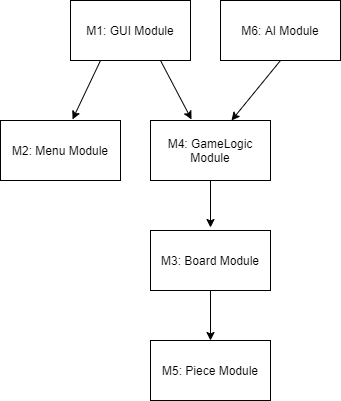
\includegraphics[width=0.7\textwidth]{UsesHierarchy.png}
\caption{Use hierarchy among modules}
\label{FigUH}
\end{figure}

%\section*{References}

\bibliographystyle {plainnat}
\bibliography {MG}

\end{document}